\documentclass{article}
\usepackage{yfonts, xcolor}
\usepackage{multicol}
\usepackage{eso-pic}
\usepackage[object=vectorian]{pgfornament}
\usepackage{geometry}
\geometry{
 a4paper,
 total={170mm,257mm},
 left=20mm,
 top=20mm,
}

% Page background taken from here: https://latex.org/forum/viewtopic.php?f=5&t=25013
% Tarot card images taken from: https://github.com/metabismuth/tarot-json

\pagenumbering{gobble}

\graphicspath{ {./Images/} }

\begin{document}

\AddToShipoutPicture{\put(0,0){\includegraphics[width=\paperwidth, height=\paperheight]{odd_page.jpg}}}

\centering{
\section*{\textgoth{\huge\underline{\textcolor{red}{E}xample of \textcolor{red}{P}lay}}}
}

\begin{multicols*}{2}

\raggedright
\textswab{1. Player 1 draws: Ace of Cups:, 4 of Swords:, 7 of Wands:, 2 of Wands: and The Fool.}

\begin{center}
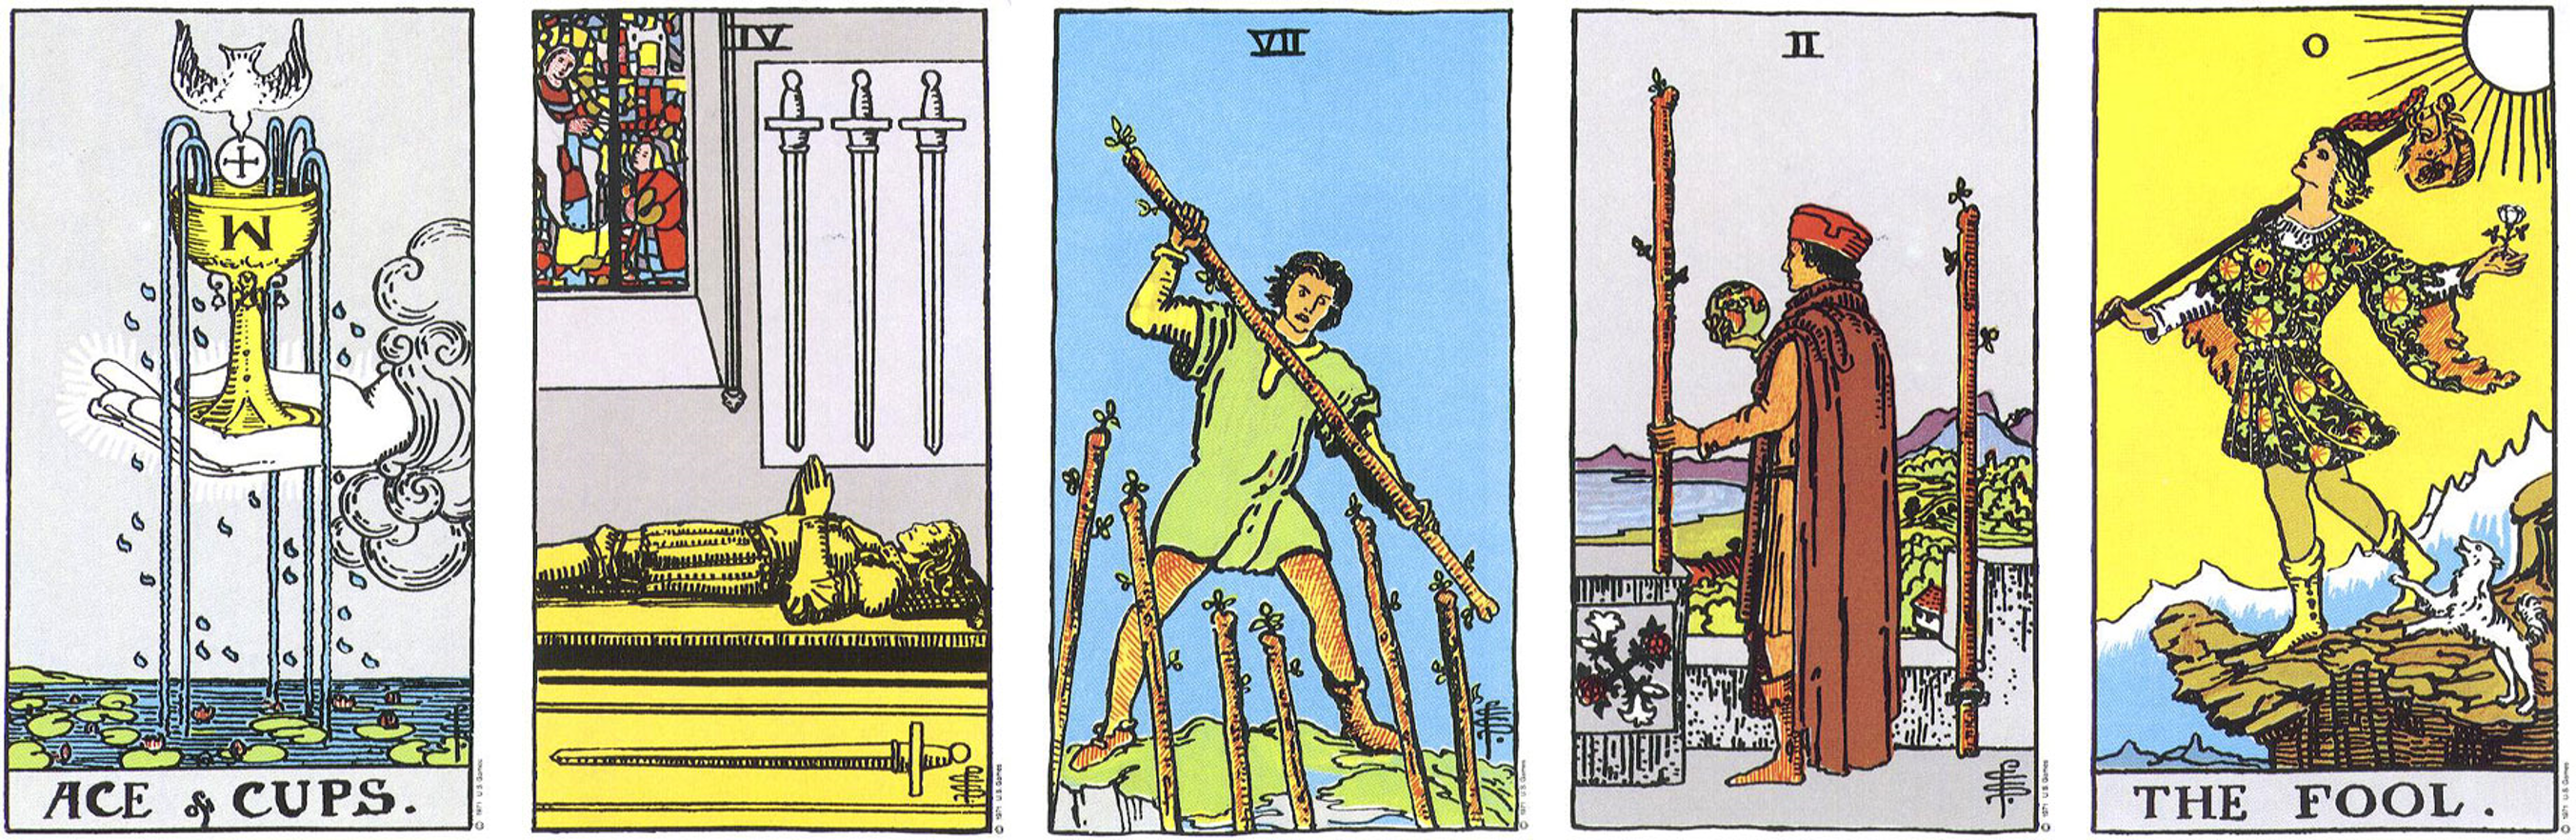
\includegraphics[scale=0.28]{Player1Hand}
\end{center}

\textswab{2. Player 2 draws: Death, The Hermit, 4 of Pentacles:, 5 of Cups: and Page of Wands:.}

\begin{center}
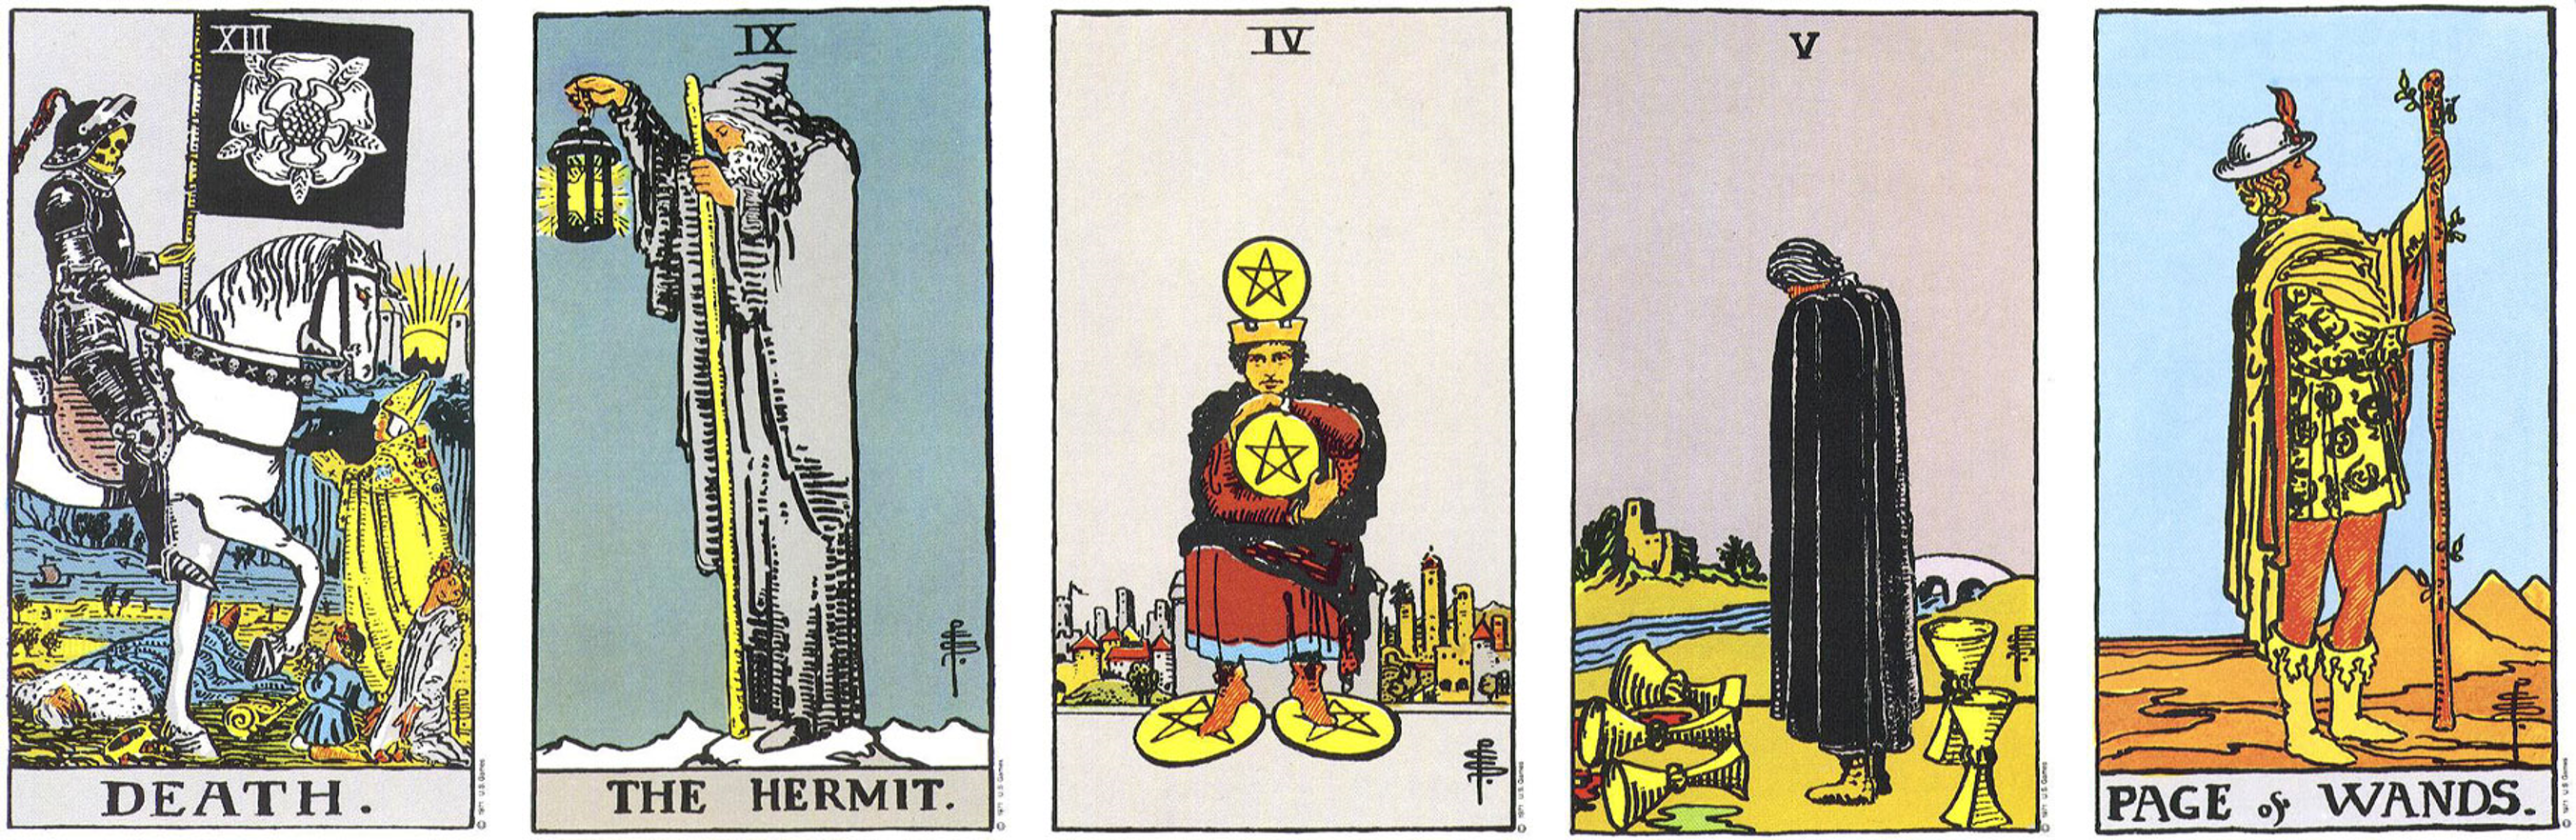
\includegraphics[scale=0.28]{Player2Hand}
\end{center}

\textswab{3. Player 1 choos:es: Ace of Cups:, 4 of Swords: and The Fool.}

\begin{center}
\includegraphics[scale=0.28]{Player1Choice}
\end{center}

\textswab{4. Player 2 choos:es: Death, The Hermit and Page of Wands:.}

\begin{center}
\includegraphics[scale=0.28]{Player2Choice}
\end{center}

\textswab{5. Both players: place their chos:en cards: face down.}

\begin{center}
\includegraphics[scale=0.28]{FaceDown}
\end{center}

\textswab{6. Player 1 wins: the coin flip and choos:es: Player 2 to reveal firs:t. Player 2 reveals: Page of Wands: (worth 10 points:).}

\begin{center}
\includegraphics[scale=0.28]{Turn1Player2}
\end{center}

\textswab{7. Player 1 reveals: Ace of Cups:. Cups: always: beat Wands: so Player 1 wins: this: round.}

\begin{center}
\includegraphics[scale=0.28]{Turn1Player1}
\end{center}

\textswab{8. Player 1 won the las:t round s:o mus:t reveal next. They choos:e 4 of Swords: (worth 4 points:).}

\begin{center}
\includegraphics[scale=0.28]{Turn2Player1}
\end{center}

\textswab{9. Player 2 reveals: The Hermit (worth 9 points:) s:o Player 2 wins: this: round.}

\begin{center}
\includegraphics[scale=0.28]{Turn2Player2}
\end{center}

% \columnbreak
\textswab{10. Each player only has: one card left, s:o both reveal s:imultaneous:ly. Player 1 reveals: The Fool (worth 0 points:) and Player 2 reveals: Death (worth 13 points:). As: both played cards: are Major Arcana, the lowes:t value wins:, s:o Player 1 wins: this: round. As: Player 1 won 2 rounds:, whils:t Player 2 only won one, Player 1 wins: the game.}

\begin{center}
\includegraphics[scale=0.28]{Turn3}
\end{center}


\end{multicols*}
\end{document}
